\begin{figure}
  \centering
  \includegraphics[width=.95\linewidth]{figures/aws-variation.pdf}
  \caption{Bandwidth measurement between Amazon EC2 sites (from Ireland to
    California).}
  \label{fig:bw}
\end{figure}

\begin{figure*}
  \centering
  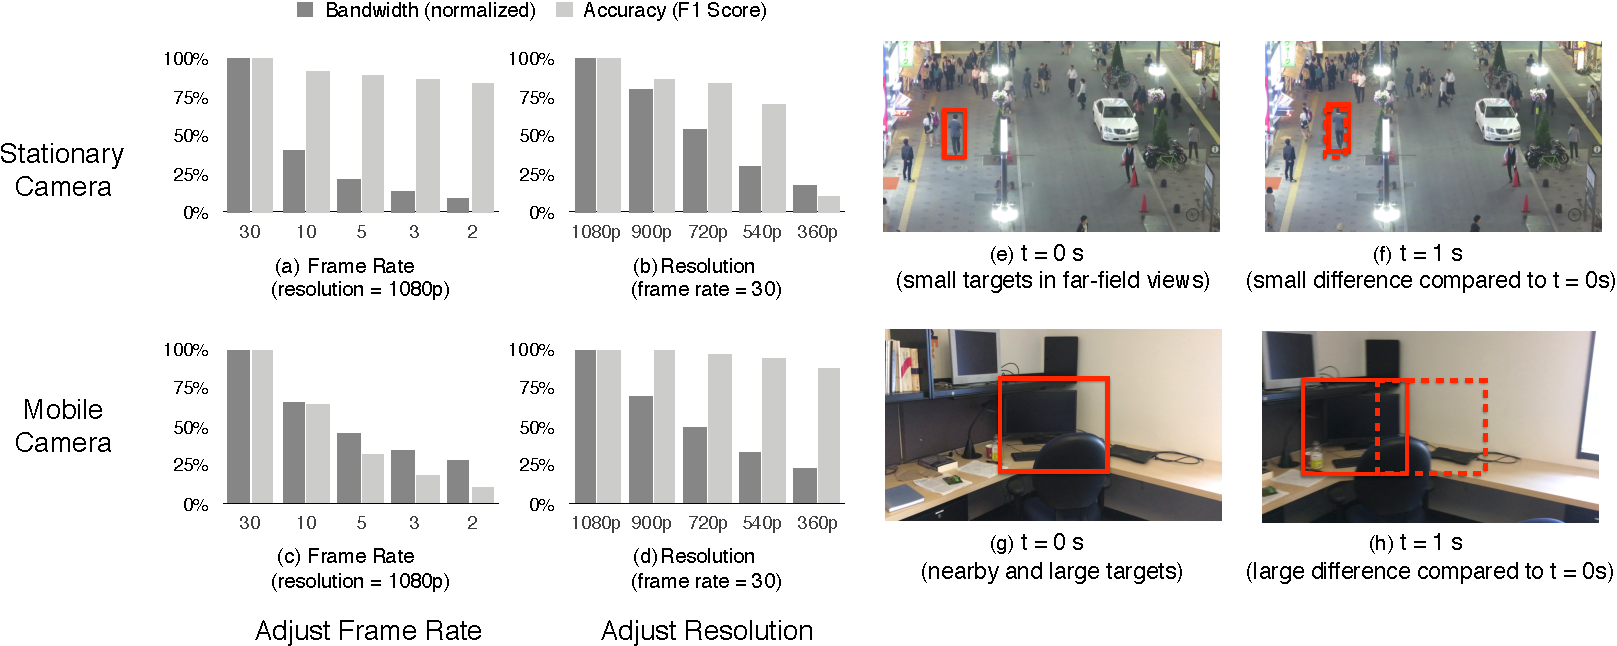
\includegraphics[width=1.0\linewidth]{figures/motiv-app-specific.pdf}
  \caption{Application-specific optimizations don't generalize. Adaptations
    designed for stationary cameras will work poorly for mobile cameras. The
    accuracy here is defined as F1 score~\cite{Rijsbergen:1979:IR:539927} for
    all detection. A detection is successful when the intersection over union
    (IOU) is larger than 50\%~\cite{everingham2010pascal}.}
  \label{fig:app-specific}
\end{figure*}

\section{Motivation}
\label{sec:motivation}

In this section, we examine the gap between high application demands and limited
wide-area bandwidth. We then show that neither application-specific
optimizations nor manual policies solve the problem.

\subsection{Wide-area Streaming Applications}
\label{sec:wide-area-streaming}

\paraf{Video Surveillance:} We envisage a city-wide monitoring system that
aggregates camera feeds (both stationary ground cameras and moving aerial
vehicles) and analyzes video streams in real-time for surveillance, anomaly
detection or business intelligence~\cite{oh2011large}. Traditionally, humans are
involved in analyzing abnormal activities. Recent advances in computer vision
and deep learning has dramatically increased the accuracy for visual scenes
analysis, such as pedestrian detection~\cite{dollar2012pedestrian}, vehicle
tracking~\cite{coifman1998real}, or facial recognition to locate people of
interest~\cite{parkhi2015deep, Lu:2015:SHF:2888116.2888245}.

\para{High-frequency IoT Sensors:} Traditionally, environmental sensors are slow
and not data-intensive~\cite{atzori2010internet}. Increasingly, high-frequency,
high-precision sensors are being deployed. For example, uPMUs monitor the
electrical grid with a network of 1000 devices; each produces 12 streams of 120
Hz high-precision values accurate to 100 ns. This amounts to 1.4 million points
per second that requires specialized time-series
database~\cite{andersen2016btrdb}.

\para{Industrial Monitoring:} Large organizations today are managing 10--100s of
data centers (DCs) and edge clusters worldwide~\cite{calder2013mapping}. While
most log analysis today runs in a batch mode and on a daily basis, there is
trend in analyzing logs in real-time for quicker optimization. For example, a
content distribution network (CDN) can improve the overall efficiency by
optimizing data placement if the access logs can be processed in real-time.

% We consider the practical issues with deploying these applications in the
% wide-area. Our stand is that these applications face a bigger network
% challenge.  Data generated from the edge often fail to be delivered to the
% processing site because of the scarce and variable bandwidth capacity in the
% wide-area. Once they arrive, existing stream processing systems can easily
% manage a large cluster and perform data analytics at real-time.

\subsection{Wide-area Bandwidth Characteristics}
\label{sec:wide-area-bandwidth}

Recent work on WAN-aware systems have all demonstrated the insufficiency and
cost nature of wide area bandwidth~\cite{pu2015low, vulimiri2015global}. Figure
2 in Gaia~\cite{hsieh17gaia} shows that the WAN bandwidth capacity is 15x
smaller than the LAN bandwidth on average, and up to 60x smaller in the worst
case.

In addition to the scarcity, WAN bandwidth also has great variability. We
conducted a day-long measurements using iPerf~\cite{iperf3} to measure the
pair-wise bandwidth between four Amazon EC2 sites. We observed large variance in
the measured bandwidth and one such pair of sites is shown
in~\autoref{fig:bw}. There are occasions that available bandwidth is below 25\%
of the maximum bandwidth.

The back-haul links between EC2 sites are better---if not at least
representative---in comparison to the general wide area links. Similar
variations have also been reported in wireless network~\cite{biswas2015large},
ISP network~\cite{grover2013peeking} and cellular
network~\cite{nikravesh2014mobile}. The scarce and varying nature poses real
challenge to the realization and successful deployment of wide-area streaming
applications.

\subsection{Making the Case for a System Approach}
\label{sec:making-case-sys-approach}

This section motivates a system-level approach by examining how the
application-specific solutions and manual policies fail to solve the problem.

\para{Application-specific solutions don't generalize.} First of all, each
analytical application has its own goal, entailing different adaptive
strategies. For example, existing solutions for video streaming focus on
end-user quality of experience (QoE)~\cite{yin2015control, michalos2012dynamic,
  pantos2016http}. When applying these techniques to machine-based video
analytics, the system will unnecessarily maintain a high frame rate.

Moreover, each algorithm in analytical applications relies on different
information from the data. For example, many computer vision detection
algorithms depends on the edge information~\cite{canny1986computational,
  lowe2004distinctive, viola2001rapid} while object tracking
applications~\cite{allen2004object} works best when the inter-frame difference
is small.

What's more, similar applications with a different context requires their own
strategy. We illustrate this point with an example in
\autoref{fig:app-specific}. In object detection deployed with a stationary
camera, when we take the pedestrians' walking speed into consideration, a high
frame rate is not necessary. But because these surveillance cameras are far from
the target, it's crucial to have a sharp image with high-resolution. On the
other hand, when running object detection with a mobile phone, due to the
movement of the camera, reducing frame rate will introduce significant errors.

\para{Manual polices are sub-optimal.} We consider manual policies for
adaptation. JetStream~\cite{rabkin2014aggregation} offers an example:
\textit{``if bandwidth is insufficient, switch to sending images at 75\%
  fidelity, then 50\% if there still isn't enough bandwidth. Beyond that point,
  reduce the frame rate, but keep the images at 50\% fidelity.''} This approach
has the following issues.

The specification is not precise. These policies are developer heuristics and
not backed up by measurements. There is no direct association of the application
accuracy with the 75\% fidelity configuration. Besides, it's unclear about how
much the policy would affect the data size. For example, reducing the frame rate
by 50\% \textit{seems} to half the data rate. But when the video is encoded with
H.264, frame rate's reduction leads to bigger inter-frame differences, resulting
in a larger P-frame size.

%% \autoref{fig:h264} illustrates this complex relationship with an example of
%% H.264 encoding under four different frame rates.

The specification is not scalable. The straw-man solution quickly leads to too
many policies when multiple dimensions are involved or a fine-grained control is
desired. Writing many policies is tedious and error-prone.

The abstraction is too low-level. Developers are forced to manually study and
measure the impact of individual operations, prohibiting its wide adoption in
practice.

%%% Local Variables:
%%% mode: latex
%%% TeX-master: "sosp17"
%%% End:
